\documentclass{article}
\usepackage[latin1]{inputenc} % un package



\begin{document}
\section{Existant Organisationnel}
    \subsection{Structure Organisationnel de GSTP}

		L'entreprise GSTP est centr\'ee autour d'un si\'ege social, il regroupe six directions :
				\begin{itemize}
        \item Direction g\'en\'erale
        \item Direction g\'en\'erale (DG)
				\item Direction des ressources humaines (DRH)
				\item Direction des finances et comptabilit\'e (DFC)
				\item Direction informatique (DI)
				\item Direction du mat\'eriel (DM)
				\item Direction travaux, \'etudes et m\'ethodes (DTEM).
    \end{itemize}
    L'entreprise poss\`ede environ une quarantaine de chantiers autonomes. Etant donn\'e que le
champ d'action se porte sur un rayon d'environ 500 km, il peut entrainer des difficult\'es logistiques
et de transport de mat\'eriel.

		% ORGANIGRAMME
		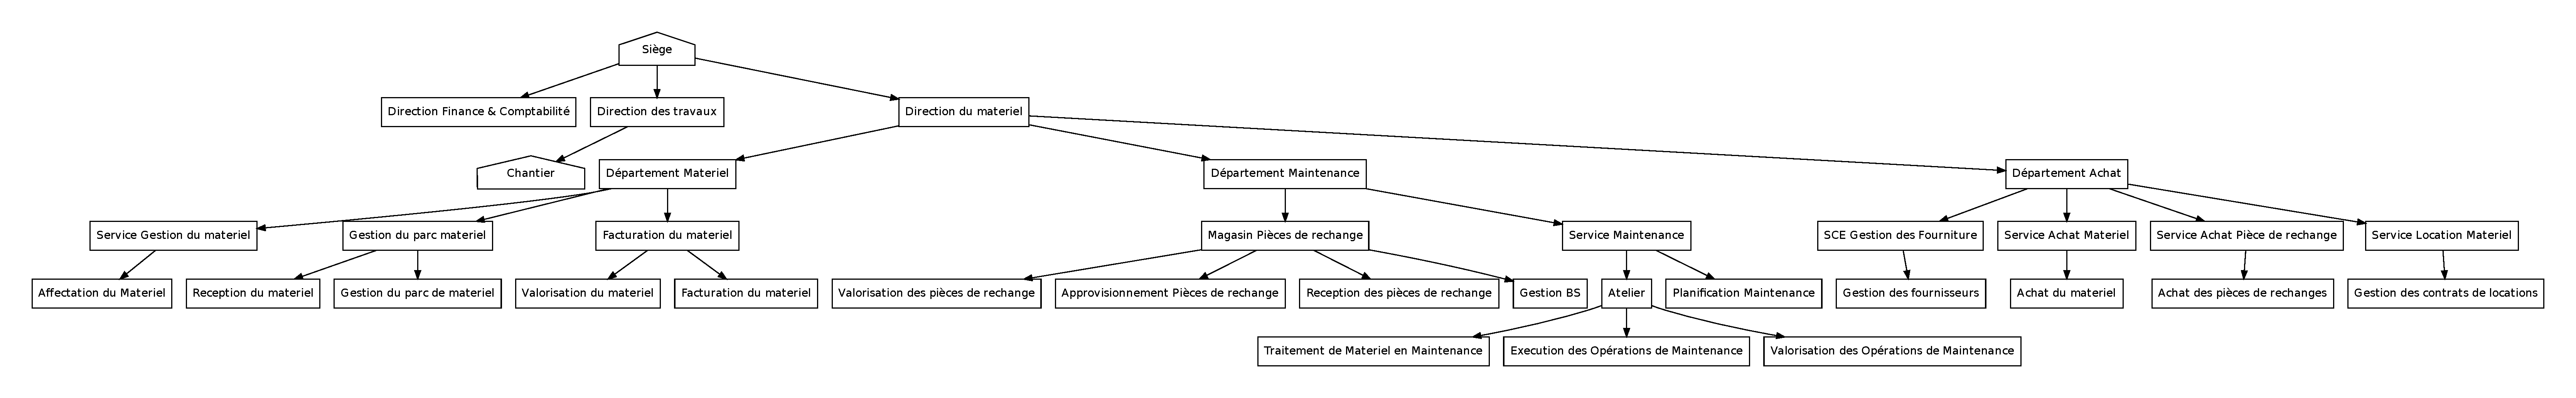
\includegraphics[width=\textwidth]{img/structureOrganisationnel.pdf} 
		
    \subsection{Direction du Materiel (DM)}
            Rattach\'ee \'a la direction g\'en\'erale, la direction du materiel a pour missions de :
            \begin{itemize}
                \item affecter le mat\'eriel aux chantiers.
                \item assurer la maintenance et la r\'enovation du mat\'eriel.
                \item g\'erer le stock de pi\`eces de rechange.
                \item renouveler le mat\'eriel (acquisition), avec l'accord de la DG car il s'agit d'un acte d'investissement.
                \item facturer l'utilisation du mat\'eriel aux chantiers. La DM joue un r\'ele de fournisseur (location du mat\'eriel) vis-\'a-vis des chantiers.
            \end{itemize}
            
        \subsubsection{Les D\'epartements et leur r\'eles}
            \paragraph{D\'epartement Materiel}
                Le d\'epartement materiel est compos\'e de trois services :
                \subparagraph{Service Gestion du Mat\'eriel}
                    Son r\^ole est de g\'erer le planning d'affectation et d'assurer l'affectation du mat\'eriel aux diff\'erents chantiers. Il est consitut\'e de trois personnes.
                \subparagraph{Gestion du Parc Mat\'eriel}
                    Il s'occupe de la r\'eception, envoi du mat\'eriel et de la gestion du parc mat\'eriel. Il est constitu\'e d'une personne.
                \subparagraph{Facturation du Mat\'eriel}
                    Ce service s'occupe de la valorisation et de la facturation du mat\'eriel. Il est constitu\'e d'une personne.        
                
            \paragraph{Departement Maintenance}
                Il est compos\'e de deux services :
                \subparagraph{Le service gestion des Pi\`eces de Rechange}
                    Son r\^ole est d'assurer l'approvisionnement, la r\'eception, la valorisation et la gestion des pi\'eces   de rechange. Il y a un magasin au si\`ege de l'entreprise et deux autres d\'elocalis\'es. Ce service est constitu\'e d'une personne par magasin. 
                \subparagraph{Le service de Maintenance}
                    Il est compos\'e d'une quarantaine d'ateliers et il s'occupe de la planification, de l'ex\'ecution et de la valorisation des op\'erations de maintenance et des divers traitements. Ce service est constitu\'e de 60 personnes r\'epartis sur 40 ateliers (dont 8 \'a l'atelier principal, et les autres \'etant repartis sur les ateliers de chantiers).

            \paragraph{Departement Achat}
                Le d\'epartement achat est constitu\'e de quatres services :

                \subparagraph{Service Gestion des Fournisseurs}
	                C'est le service qui va \^etre en communication avec les fournisseurs de mat\'eriel afin d'avoir les meilleurs mat\'eriels sur le march\'e aux moindres co\^uts.
                \subparagraph{Service d'Achat du Mat\'eriel}
	                Ce service s'occupe des achats de nouveaux mat\'eriels.
                \subparagraph{Service d'Achat des pi\`eces de Rechange}
	                Ce service s'occupe de tous les achats de pi\`eces de rechange.
                \subparagraph{Service Location du Mat\'eriel}
	                Ce service s'occupe des locations de mat\'eriels lorsque le parc n'offre pas suffisamment de disponibilit\'es pour r\'epondre \'a un besoin d'un chantier. Il peut \'egalement s'occuper de l'achat d'autres prestations (maintenance, etc.)


\section{Processus strat\'egiques}
		La direction mat\'eriel de GSTP repose sur 5 principaux processus :
		\begin{itemize}
				\item Processus d'approvisionnement de pieces de rechange
				\item Processus de facturation du materiel pour un chantier
				\item Processus d'affectation et de restitution du materiel
				\item Processus de maintenance du materiel
				\item Processus de planification de l'affectation du materiel
    \end{itemize}


		\subsection{Processus d'approvisionnement de pieces de rechange}
				\subsubsection{Description}
				
						L'approvisionnement des pi\'eces de rechange se d\'eroule suivant le cycle suivant :
						\begin{itemize}
						    \item D'abord on calcule le stock des pi\`eces de rechange \'a chaque fois que l'on fait l'inventaire mensuel des pi\`eces de rechange ou lorsque l'on re�oit des pi\`eces de rechange, ou lorsqu'une pi\`ece de rechange sort du stock (magasin).
						    \item On produit ainsi la variation de stock qui, associ\'ee aux pr\'evisions de consommation nous conduit \'a calculer les besoins en pi\'eces de rechange. Un calcul des besoins est \'egalement fait mensuellement. Le calcul des nouveaux besoins donne suite \'a l'\'edition d'une demande de r\'eapprovisionnement en pi\`eces de rechange.
						    \item Enfin on transmet cette demande de r\'eapprovisionnement (ou une demande urgente d'approvisionnement
\'etablie par un des chantiers), cela aura pour effet de produire une commande de pi\`eces de rechange par le d\'epartement Achat.
						\end{itemize}
						
				%\subsubsection{MCD}
				
				%\subsubsection{MCT}
				
				%\subsubsection{MOT}
				
		\subsection{Processus de facturation du materiel pour un chantier}
				\subsubsection{Description}
				
				Cette proc\'edure permet de facturer en interne le mat\'eriel sur les diff\'erents chantiers. Cette t\'ache n'est pas assur\'ee par le service Achat car celui-ci ne s\'eoccupe que des factures ext\'erieures.
				\newline
				L'edition de la facturation d'utilisation du materiel par les chantiers est calculee par le service
Facturation Materiel du departement Materiel en fonction du :
				\begin{itemize}
						    \item Releve mensuel du fonctionnement du materiel (RMFM) etabli par les chantiers,
						    \item Releve mensuel des heures de main d'oeuvre (RMHMO) etabli par le service Maintenance
du departement Maintenance,
						    \item Releve mensuel de consommation de pieces de rechange et pneus (RMCPR) etabli par le Service de Gestion de Pieces de Rechange du departement Maintenance,
						    \item des frais de gestion, de la masse salariale et du cout de l'heure de main d'oeuvre de la
direction de Materiel (DM), renseignements fournis par la direction des Finances et Comptabilite (DFC).
				\end{itemize}
				
				%\subsubsection{MCD}
				
				%\subsubsection{MCT}
				
				%\subsubsection{MOT}

		\subsection{Processus d'affectation et de restitution du materiel}
				\subsubsection{Description}
				
				Cette proc\'edure g\`ere la pr\'esence de mat\'eriel sur site depuis sa r\'eception aupr\`es du fournisseur jusqu\'a son retour du chantier.
				\newline
				La proc\'edure d'affectation s'effectue g\'en\'eralement sur la base du planning d'affectation qui correspond aux pr\'evisions d'utilisation du mat\'eriel \'etabli par le DTEM. D'autres demandes, non pr\'evues au planning, sont \'emises par les chantiers. Ces demandes sont satisfaites, notamment par la sous-traitance. 
				\newline
				En effet, si un mat\'eriel venait \'a manquer, l'entreprise effectue des locations aupr\`es d'entreprises sp\'ecialis\'ees dans la location de mat\'eriel BTP. Lorsque le mat\'eriel n'est plus n\'ecessaire sur le chantier, un avis de restitution de mat\'eriel est envoy\'e, on contr\'ele l'\'etat du mat\'eriel; s'il est en bon \'etat, une demande d'entr\'ee est demand\'ee au service Gestion du parc mat\'eriel; s'il \'etait en location, il est dirig\'e vers le service location du mat\'eriel; et s'l est en panne, une demande de maintenance est faite au service Maintenance.


				%\subsubsection{MCD}
				
				%\subsubsection{MCT}
				
				%\subsubsection{MOT}
				
		\subsection{Processus de maintenance du materiel}
				\subsubsection{Description}
				
				Le d\'epartement de gestion de la maintenance se charge de la maintenance pr\'eventive du mat\'eriel (r\'evisions \'e la restitution par un chantier ou selon le planning de maintenance), et de sa r\'enovation. Lorsqu\'eil y a une panne, elle peut \^etre diagnostiqu\'ee sur place pour savoir s'il faut r\'eparer sur le chantier ou rapatrier le mat\'eriel au si\'ege.
				\newline
				Le service de gestion de la maintenace s'occupe de planifier les op\'erations de maintenance, les ex\'ecuter. Elle est compos\'ee de soixante personnes r\'eparties sur quarante ateliers. Huit d'entres elles sont sur l'atelier principal, et le reste sur les ateliers de chantier. Lorsqu'une op\'eration de maintenance est lanc\'ee, des personnes sont affect\'ees et des pi\`eces de rechange sont command\'es, puis la r\'eparation est effectu\'ee. A la fin de chaque op\'eration de maintenance un avis de maintenance est \'emis au d\'epartement maintenance ou au chantier concern\'e.
				
				%\subsubsection{MCD}
				
				%\subsubsection{MCT}
				
				%\subsubsection{MOT}
				
		\subsection{Processus de planification des affectation du materiel}
				\subsubsection{Description}
				
				Ce processus est tr\`es transverse aux d\'epartements et services de la direction mat\'eriel.
				Parmi les services qui r\'ealisent la planification, il y a : ceux du d\'epartement achats (les services d'achat du mat\'eriel, d'achat de pi\'eces de rechanges et location du mat\'eriel), ceux \'egalement des d\'epartements mat\'eriel et de maintenance.
				\newline
				Le d\'epartement de mat\'eriel planifie l'utilisation de mat\'eriel par les chantiers et leurs affectations aux chantiers. Elle s'occupe d'envoyer aux d\'epartements achat et maintenance les demandes de mat\'eriel par chantier : demande de location ou d'achat de nouveau mat\'eriel et planification des op\'erations de maintenance du mat\'eriel sur site.
				\newline
				Le d\'epartement d'achat du mat\'eriel pr\'evoit un planning de commande de mat\'eriel et la location de celui-ci. 
				\newline
				Le d\'epartement de maintenance planifie la maintenance, la disponibilit\'e du personnel et la consommation de pi\'eces de rechange.
				
				%\subsubsection{MCD}
				
				%\subsubsection{MCT}
				
				%\subsubsection{MOT}

\section{Existant informatique}

		Actuellement, 30 chantiers effectuent leur pointage manuel et ensuite les transmettent au si\'ege. Seuls 10
chantiers sont \'equip\'es d'ordinateurs. L'entreprise pr\'evoit d'\'equiper l'ensemble des chantiers sur un horizon de 10 mois. 
Ces outils informatiques permettent la saisie et la transmission des donn\'ees de gestion vers le si\`ege.
		Au si\'ege, il y a 60 postes et une imprimante principale.
		
		\subsection{Niveau logiciel}
		
		Au niveau de la direction du mat\'eriel, l'architecture logicielle regroupe plusieurs applications.
Chaque d\'epartement de la DM poss\`ede des applications en interne et ind\'ependantes qui reposent sur des fichiers. Aucun syst\'eme informatique
ne permet la centralisation de ces informations.

		\begin{description}
			\item[D\'epartement Mat\'eriel :] poss\`ede une application de gestion du planning ainsi qu'une application de facturation.
			\item[D\'epartement Maintenance :] dispose d'un logiciel estion de stocks et pi\`eces de r\'echange, et d'un autre de planification de maintenance
			\item[D\'epartement Achat :] poss\`ede une applications de gestion des fournisseurs (300 environ), d'une autre de gestion de bons de commande.
		\end{description}


		\subsection{Niveau mat\'eriel}

		 L'architecture mat\'erielle de la DM n'est pas tr\`es d\'evelopp\'ee.

		\begin{description}
			\item[D\'epartement Mat\'eriel :] est dot\'e de 3 postes et 2 imprimantes.
			\item[D\'epartement Maintenance :] est dot\'e de 2 postes et 2 imprimantes
			\item[D\'epartement Achat :] est dot\'e de 2 postes et 2 imprimantes
		\end{description}
		
		
		
\section{Dysfonctionnements}	
		
		Au niveau de l'existant organisationnel, les dysfonctionnements d\'etect\'es sont :
		
		\subsection{D\'epartement Mat\'eriel}
				\begin{itemize}
						\item Mauvaise planification des affectations du mat\'eriel car le dispositif de pointage ne permet pas d'avoir une vision globale du planning.
						\item Immobilisation du mat\'eriel car le syst\'eme actuel ne permet pas de r\'eperer en temps r\'eel l'inexploitation d'un mat\'eriel.
						\item L'utilisation du papier, en plus d'\^etre un moyen peu fiable, constitue une perte de temps cons\'equence dans le processus de transmission de l'information au si\'ege emp\'echant une gestion temps r\'eel du mat\'eriel.
						\item Les r\'elev\'es mensuels d'exploitation du mat\'eriel, des heures de main d'oeuvre et de consommation de pi\'eces de rechange ne sont disponibles qu'\'e la fin du moins. Ce qui engendre une perte importante du temps et une charge de travail importante durant une p\'eriode tr\`es r\'eduite.
				\end{itemize}
		
		\subsection{D\'epartement Maintenance}
				\begin{itemize}
						\item Une mauvaise gestion des stocks de pi\`eces de rechange car elle n'int\`egre pas une anticipation des maintenances planifi\'ees et des demandes de maintenances urgentes.
						\item L\'eimmobilisation du stock engendre des frais suppl\'ementaires.
						\item Le departement de maintenance ne g\`ere pas son personel de mani\`ere autonome car la plupart (52 personnes sur 60) sont repartis sur des ateliers de chantiers.
				\end{itemize}
		
		\subsection{D\'epartement Achat}
				\begin{itemize}
				    \item Absence d'\'etude pr\'evisionnelle, simulation , statistique des mat\'eriels les plus utilis\'es, lou\'es, ce qui aurait permis d'\'elaborer un planning pr\'evisionnel des besoins en gros mat\'eriel et pi\'eces de rechange. L'abscence d'un tel planning emp\'eche les fournisseurs de pr\'evoir leurs stocks de produits (stocks de s\'ecurit\'e), ce qui pourrait entra\'ener des retards de livraisons des fournisseurs et par cons\'equent r\'eduire les temps de r\'eponse aux demandes (notamment celles urgentes) des chantiers.
						\item Le trop grand nombre de fournisseurs (300), entra\^ine une lenteur au niveau du choix du fournisseur, ce qui ralentit aussi le processus d'achat, en plus du fait de ne pas disposer de fournisseurs fid\'elis\'es afin de b\'en\'eficier de r\'eduction de prix. On pourrait fid\'eliser les fournisseur selon la qualit\'e de leurs produits et leurs prix, mais aussi selon la proximit\'e g\'eographique, ce la permettrait d'amortir les frais de transport.
						\item L'absence d'un syst\`eme de centralisation des demandes d'achat et de r\'enovation du gros mat\'eriel aux pr\'es de la DG, afin d'acc\'elerer le processus d'aquisition et de r\'epondre rapidement aux demandes des chantiers.
				\end{itemize}
		
		Concernant l'existant informatique, nous avons remarqu\'e les dysfonctionnements suivants :
		\begin{itemize}
				\item Ind\'ependance totale des applications des d\'epartements de la DM et le manque de communication entre elles.
				\item Inexistance d'un syst\`eme informatique permmetant de centraliser les informations et g\'erer la communication entre le siege et les chantiers.
				\item Utilisation du papier, qui est un moyen peu fiable et constitue une perte de temps cons\'equence dans le processus de transmission de l'information au si\`ege, engendrant un r\'eel manque de performance et de qualit\'e.
				\item Les traitements et les donn\'ees sont sur un m\^eme serveur, ce qui peut poser un gros probleme en cas de panne.
				\item Aucune de strategie de sauvegarde et de gestion des historiques malgr\'e les grands flux donn\'ees trait\'es.
				\item Aucune strategie au niveau de la securite de l'information.
		\end{itemize}

		Les moyens et \'equipements utilis\'es au sein de l'entreprise GSTP sont r\'eellements insuffisants pour r\'epondre \'e ces processus complexes, et entrainent un r\'eel manque de performance. Actuellement, l'existant informatique ne peut pas de permettre de r\'epondre aux attentes de
GSTP au niveau de l'am\'elioration de la qualit\'e, de la performance � tous les niveaux et la r\'eduction des co�ts.
		
\end{document}
